%
%  order report template
%
%  Created by Matthias Laug on 2009-08-06.
%
\documentclass[a4paper]{article}


\renewcommand{\baselinestretch}{1.3}

% set font to times
\usepackage{mathptmx}
\usepackage[scaled=1]{helvet}

\renewcommand\familydefault{phv}

% set margins 
\usepackage[left=20mm, right=20mm, top=20mm, bottom=40mm] {geometry}

% Use utf-8 encoding for foreign characters
%\usepackage[applemac]{inputenc}
\usepackage[utf8]{inputenc}

% Use german language
\usepackage[german]{babel}

% Setup for fullpage use
% multirow - rowspan in tables
% graphicx - include graphics
% fancyhdr - footer/header
% booktabs - nice tables
\usepackage{multirow, graphicx, fancyhdr, booktabs,array,colortbl}

% define \EUR{amount}
\usepackage[right]{eurosym}

%booktabs settings
\newcolumntype{V}[1]{
	 >{\bfseries\huge}p{#1}
} 							% tabellen�berschriften
\newcolumntype{T}[1]{
	>{\bfseries\large}p{#1}
} 							% tabellen�berschriften
\newcolumntype{v}[1]{
	>{\raggedright}p{#1}
} 							% verwende v{Xcm} f�r linksb�ndige Spalten fester Breite
\newcolumntype{w}[1]{
	>{\raggedleft}p{#1}
} 							% verwende w{Xcm} f�r rechtsb�ndige Spalten fester Breite
\newcolumntype{x}[1]{
	>{\centering}p{#1}
} 							% verwende x{Xcm} f�r zentrierte Spalten fester Breite

% Define user colors using the RGB model
	\definecolor{black}{rgb}{0,0,0}

%-------------------------------- Kopf- und Fuzeile
\pagestyle{fancy}
\fancyhf{}
\setlength{\parindent}{0pt} 
%header
%\fancyhead[C]{
\includegraphics[scale=0.5]{../pdf/header_check.jpg}}
%\fancyhead[C]{
\includegraphics[scale=0.5]{../pdf/header.eps}}
\fancyhead[R]{
\includegraphics[scale=0.5]{../pdf/yourdelivery.jpg}}
%\fancyhead[L]{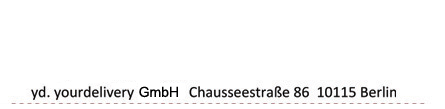
\includegraphics[scale=0.5]{../pdf/address.jpg}}

\renewcommand{\headrulewidth}{0pt}

% footer
\fancyfoot[L]{}
\fancyfoot[C]{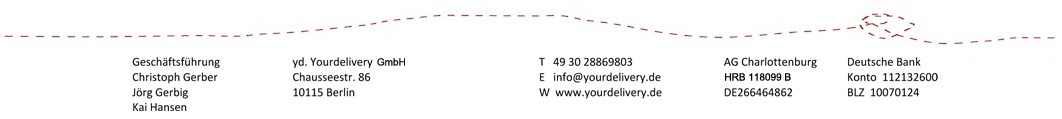
\includegraphics[scale=0.5]{../pdf/footer_only.jpg}}
%\fancyfoot[C]{
\includegraphics[scale=0.6]{../pdf/footer.eps}}
\fancyfoot[R]{}


%-------------------------------- content
\begin{document}
	
    % Bestellinformationen
		\begin{tabular}{v{0.5\textwidth}w{0.3\textwidth}r}
		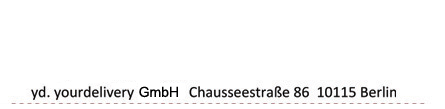
\includegraphics[scale=0.5]{../pdf/address.jpg}

		         	       	\textrm{sportme GmbH}\\
		         		\textrm{Chauseestr. 86}\\
				\textrm{10115 Berlin}\\
				\textrm{Deutschland}\\
				
				& \\
		\end{tabular}
                %add all members from group

                %add all members who will share their budget
            
            	\vspace{1.5cm}
	
		\begin{tabular}{v{0.7\textwidth}r}
				\begin{large}
					Rechnung: \textbf{RE-94589489}
				\end{large}
				&  Berlin, den {\today} \\
				\vspace{0.3cm}
				\begin{small}
					sportme GmbH Kostenstelle 9061, 9083
				\end{small}
				& \\
				\begin{small}
					F"ur die Vermittlung von Speisen und Getr"anken stellen wir Ihnen in Rechnung:
				\end{small}
				& \\ \\ 
				
				\rowcolor{black}
				\color{white} \textbf{Kostenstelle:} & \color{white} \textbf{9061, 9083} \\
				
				
				Netto gesamt:		& \EUR{120,00} \\
				\hline
				Netto  7 \%:		& \EUR{20,00} \\
				Netto 19 \%:		& \EUR{100,00} \\
				MwSt 7 \%:		& \EUR{1,40} \\
				MwSt 19 \%:		& \EUR{19,00} \\
				  \hline
				Brutto:			& \EUR{140,40} \\
				  \hline
				Bereits bezahlt:		& \EUR{100,00} \\
				  \hline
				\textbf{Offener Rechnungsbetrag:}& \textbf{\EUR{40, 40}} \\
				  \hline  \hline
				
		\end{tabular}
		\\ \\ \\
		
		Bitte "uberweisen Sie den offenen Rechnungsbetrag unter Angabe der Rechnungsnummer auf folgendes Konto:
		\begin{center}
			\begin{tabular}{v{3cm}l}
				\multicolumn{2}{v{5cm}}{yd. yourdelivery GmbH}\\
				Kontonummer: & 11 21 32 600 \\
				Banklietzahl:	& 100 701 24 \\
				& Deutsche Bank Berlin\\
			\end{tabular}
		\end{center}
		Eine genaue Auflistung der Leistungen entnehmen Sie bitte dem Anhang. Die Zahlung ist sofort f"allig.
		
		\vspace{0.5cm}
		
			
\includegraphics[scale=0.5]{../pdf/unterschrift.jpg}
		
		
		
		\newpage
		
		\begin{large}
			Rechnung: RE-94589489\\
		\end{large}
		\begin{small}
			Kostenstelle 9061, Zeitraum: 14.09.2009 - 31.10.2009\\
		\end{small}
			
		
		
		% SECOND PAGE
			%\begin{tabular}[ht]{p{0.9\textwidth}r}
			\begin{tabular}{v{0.9\textwidth}r}
				\rowcolor{black}
				\color{white} \textbf{Kostenstelle:} &  \color{white} \textbf{9061} \\
				
				Netto gesamt:		& \EUR{120,00} \\
				\hline
				Netto  7 \%:		& \EUR{20,00} \\
				Netto 19 \%:		& \EUR{100,00} \\
				MwSt 7 \%:		& \EUR{1,40} \\
				MwSt 19 \%:		& \EUR{19,00} \\
				  \hline
				Brutto:			& \EUR{140,40} \\
				  \hline
				Bereits bezahlt:		& \EUR{100,00} \\
				  \hline
				\textbf{Offener Rechnungsbetrag:}& \textbf{\EUR{40, 40}} \\
				  \hline  \hline
			\end{tabular}
			
			\vspace{1cm}
			
			\begin{tabular}{v{0.9\textwidth}r}
				\rowcolor{black}
				\color{white} \textbf{WB:} &  \color{white} \textbf{9061} \\
				
				WB Netto gesamt:		& \EUR{120,00} \\
				\hline
				Netto  7 \%:			& \EUR{20,00} \\
				Netto 19 \%:			& \EUR{100,00} \\
				MwSt 7 \%:			& \EUR{1,40} \\
				MwSt 19 \%:			& \EUR{19,00} \\
				  \hline
				WB Brutto:			& \EUR{140,40} \\
				  \hline
				Bereits bezahlt:			& \EUR{100,00} \\
				  \hline
				\textbf{WB Offener Rechnungsbetrag:}& \textbf{\EUR{40, 40}} \\
				  \hline  \hline
			\end{tabular}
			
			\vspace{1cm}
			
			\begin{tabular}{v{0.9\textwidth}r}
				\rowcolor{black}
				\color{white} \textbf{NWB:} &  \color{white} \textbf{9061} \\
				
				NWB Netto gesamt:		& \EUR{120,00} \\
				\hline
				Netto  7 \%:			& \EUR{20,00} \\
				Netto 19 \%:			& \EUR{100,00} \\
				MwSt 7 \%:			& \EUR{1,40} \\
				MwSt 19 \%:			& \EUR{19,00} \\
				  \hline
				NWB Brutto:			& \EUR{140,40} \\
				  \hline
				Bereits bezahlt:			& \EUR{100,00} \\
				  \hline
				\textbf{NWB Offener Rechnungsbetrag:}& \textbf{\EUR{40, 40}} \\
				  \hline  \hline
			\end{tabular}

			\vspace{1cm}
			
			\begin{tabular}{v{0.9\textwidth}r}
				\rowcolor{black}
				\color{white} \textbf{Kostenstelle:} &  \color{white} \textbf{9061} \\
				
				NWB Netto gesamt:		& \EUR{120,00} \\
				\hline
				WB Netto gesamt:		& \EUR{20,00} \\
				\hline
				NWB Netto gesamt:		& \EUR{100,00} \\
				\hline
				WB anteilig in \%:		& \EUR{1,40} \\
				\hline
				NWB anteilig in \%:		& \EUR{19,00} \\
			\end{tabular}
\end{document}